\documentclass{article} \usepackage{amsmath} \usepackage{amssymb} \usepackage{amsthm} \usepackage[margin=0.2in]{geometry} \usepackage{hyperref} \usepackage{physics} \usepackage{tikz} \usepackage{mathtools} \mathtoolsset{showonlyrefs} \theoremstyle{definition} \newtheorem{theorem}{Theorem}[section] \newtheorem{corollary}{Corollary}[theorem] \newtheorem{lemma}[theorem]{Lemma} \newtheorem{definition}{Definition}[section] \author{Connor Duncan} \date{\today}
\title{Physics-105-Lecture-Notes-01-24-2019}
\begin{document}
\maketitle\tableofcontents
\noindent\abstract{A single PDF with all lectures in a single document can be downloaded at \url{https://www.dropbox.com/sh/8sqzvxghvbjifco/AAC9LoSRnsRQDp7pYedgWpQMa?dl=0}. The password is 'analytic.mech.dsp'.
 This file was automatically generated using a script, so there might be some errors. If there are, you can contact me at \url{mailto:ctdunc@berkeley.edu}.}
\subsection{More orthogonal transformations} \subsubsection{Group!} Orthogonal transformation $\Lambda$ from coordinate system $S\rightarrow S'$, form a group, so that $\forall \Lambda, W$, \begin{center} \begin{tabular}{c} $\Lambda W\neq W\Lambda$\\ $\Lambda\Lambda^\dag=I_n$\\ $\Lambda_{ij}W_{jk}\neq W_{ij}\Lambda{jk}$ \end{tabular} \end{center} the reason that we care it's a group is because it's closed under multiplication, i.e. for any orthogonal transformation $\Lambda, W$, their product $W\Lambda$ is also an orthogonal transformation. \subsubsection{$\det\Lambda=1\Leftrightarrow\Lambda$ has eigenvalues=1} \begin{align} (\Lambda-I)\Lambda^\dag=1-\Lambda^\dag=(1-\Lambda)^\dag\\ \end{align} Now, solve $||\Lambda_{ij}-a\delta_ij||=0$ \begin{align} ||\Lambda-1||\cdot||\Lambda^\dag||=||(1-\Lambda)^\dag||=||1-\Lambda||\\ \therefore\\ ||\Lambda-1||=||1-\Lambda||\rightarrow||\Lambda-1||=0 \end{align} Where here, $1,I$ are used interchangeably to represent identity Consider operator $P|P_{ij}=\begin{bmatrix}-1 &0&0\\0&-1&0\\0&0&-1\end{bmatrix}$, it's the inversion operator, takes any vector $\vec{r}=(x,y,z)\rightarrow(-x,-y,-z)$. Determinant is $-1$, which allows $P$ to be unitary (i.e. $P^2$=1) We can now write any transformation $\Lambda$ as a combination of rotation and inversion. Take $W=P\Lambda$, where $W$ is a rotation matrix, since $||W||=||\Lambda||||P||=1$, then $PW=PP\Lambda=\Lambda$. \subsubsection{Eigenvectors} Consider the transformation \begin{align} \begin{bmatrix} -1.5 & 1\\ 1 & -1.5 \end{bmatrix} \end{align} \begin{center} 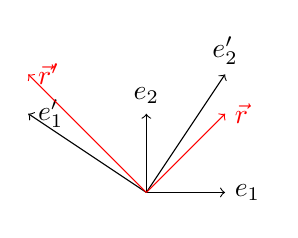
\begin{tikzpicture} \draw[->] (0,0)--(1,0) node[anchor=west]{$e_1$}; \draw[->] (0,0)--(0,1) node[anchor=south]{$e_2$}; \draw[->] (0,0)--(-1.5,1) node[anchor=west]{$e_1'$}; \draw[->] (0,0)--(1,1.5) node[anchor=south]{$e_2'$}; \draw[->,red](0,0)--(1,1) node[anchor=west]{$\vec{r}$}; \draw[->,red](0,0)--(-1.5,1.5) node[anchor=west]{$\vec{r}'$}; \end{tikzpicture} \end{center} We can consider either transformations of coordinate systems (i.e. basis vectors $e_1,e_2$) or of individual vectors ($\vec{r}$). \subsection{Rigid Body Motion} \subsubsection{Vector Product (Cross)} Take vectors $a_1,a_2$ in the coordinate system defined with basis vectors $e_1, e_2, e_3$, so that $a_1=(a_{11},a_{12},a_{13})$ and $a_2$ defined similarly. \begin{align} |\vec{a_1}\times\vec{a_2}|=|\vec{a_1}|\cdot|\vec{a_2}|\sin(\theta) \end{align} Where $\theta$ is the angle between the two vectors. When $S=\text{span}(\{e_1,e_2,e_3\})$, and is orthogonal basis. \begin{align} e_1\times e_2=e_3 && e_2\times e_3=e_1 && e_3\times e_1=e_2 \end{align} \paragraph{Levi-Civita tensor density} defined by $[e_i\times e_j]=\epsilon_{ijk}e_k$, we can write the cyclic permutations of 1,2 and 3 to get the above identities regarding $S$. We can also find the area of a parallelogram formed by two vectors $a_1, a_2$, it will be the square of the magnitude of the cross of these two vectors: $A=|a_1\times a_2|^2$. We can also calculate this using \begin{align} (a_1\times a_2)=\left|\left|\begin{matrix}a_{11} & a_{12}\\ a_{21} & a_{22}\end{matrix}\right|\right|=\det(a)e_3 \end{align} \subsubsection{Scalar Triple Product?} This man lectures very rapidly with lots of subscripts. Where's the professor? I'm pretty sure he's talking about the scalar triple product rn. Want to prove that $\epsilon_{\alpha\beta\gamma}=\epsilon_{ijk}\Lambda_{\alpha i}\Lambda_{\beta j}\Lambda_{\gamma k}$. Alternatively we can show that $||\det A||\epsilon_{\alpha\beta\gamma}=\epsilon_{ijk}A_{\alpha i}A_{\beta j}A_{\gamma k}$. \begin{align} a_3\cdot(a_1\times a_2)=V=||a_{ij}||=\left|\left|\begin{matrix}a_{11} & a_{12} & 0\\ a_{12} & a_{22} & 0\\0&0&0\end{matrix}\right|\right| \end{align} \textbf{double check that those zeroes are there}. His handwriting was kind of scratchy here. Here's probably a better example \url{https://en.wikipedia.org/wiki/Triple_product} Also, $a\times(b\times c)=b(a\cdot c)-c(a\cdot b)$, to be proven at home. \section{Newtonian Physics} \subsection{Angular Velocity} Reintroduce angular velocity. Consider $\vec{r}$, with $\Lambda_{ij}=\delta_{ij}+\delta\varphi_{ij}$, with $\delta\varphi<<1$. We still want $\Lambda$ to be unitary ($\Lambda\Lambda^\dag=1$), so \begin{align} (1+\delta\varphi)(1+\delta\varphi^\dag)=1 1+\delta\varphi+\delta\varphi^\dag+\delta\varphi\delta\varphi^\dag=1 \end{align} We know that $\delta\varphi=-\delta\varphi^\dag$, since $\delta\varphi\delta\varphi^\dag$ is very very small. Now consider $x'=(1+\delta\varphi)x$. We can take \begin{align} x'-x=\delta\varphi x\\ \delta x= \begin{bmatrix} 0 & -\delta\varphi_3 & \delta\varphi_2\\ 0 & 0 & -\delta\varphi_1\\ 0 & 0 & 0 \end{bmatrix}\\ \delta x=(\delta\varphi\times x) \end{align} In other words, $\delta r=[\delta\varphi\times r]$. Then, $\pdv{x}{t}=(\pdv{\phi}{t}\times x\Rightarrow\dv{r}{t}=[\Omega\times r]$ where $\Omega$ is the \emph{Angular Velocity}. \subsection{Linear Velocity} It's the time derivative of position. In arbitrary coordinates it's expressed simply \begin{align} \dv{r}{t}=\lim_{\Delta t\rightarrow0}\frac{r(t+\Delta t)-r(t)}{\Delta t} \end{align} In cartesian coordinates it simplifies to the sum of the componentwise time derivatives. \subsection{Coordinate Transform w/ AV} Relations of coordinate transformation with some from $S$ that has a very complicated motion compared to frame $S'$. \begin{equation} \left(\dv{r}{t}\right)_S=\left(\dv{r}{t}\right)_{S'}+(\Omega\times r) \end{equation}
\end{document}
